\begin{figure}[t]
  \centering
  \vspace{2mm}
  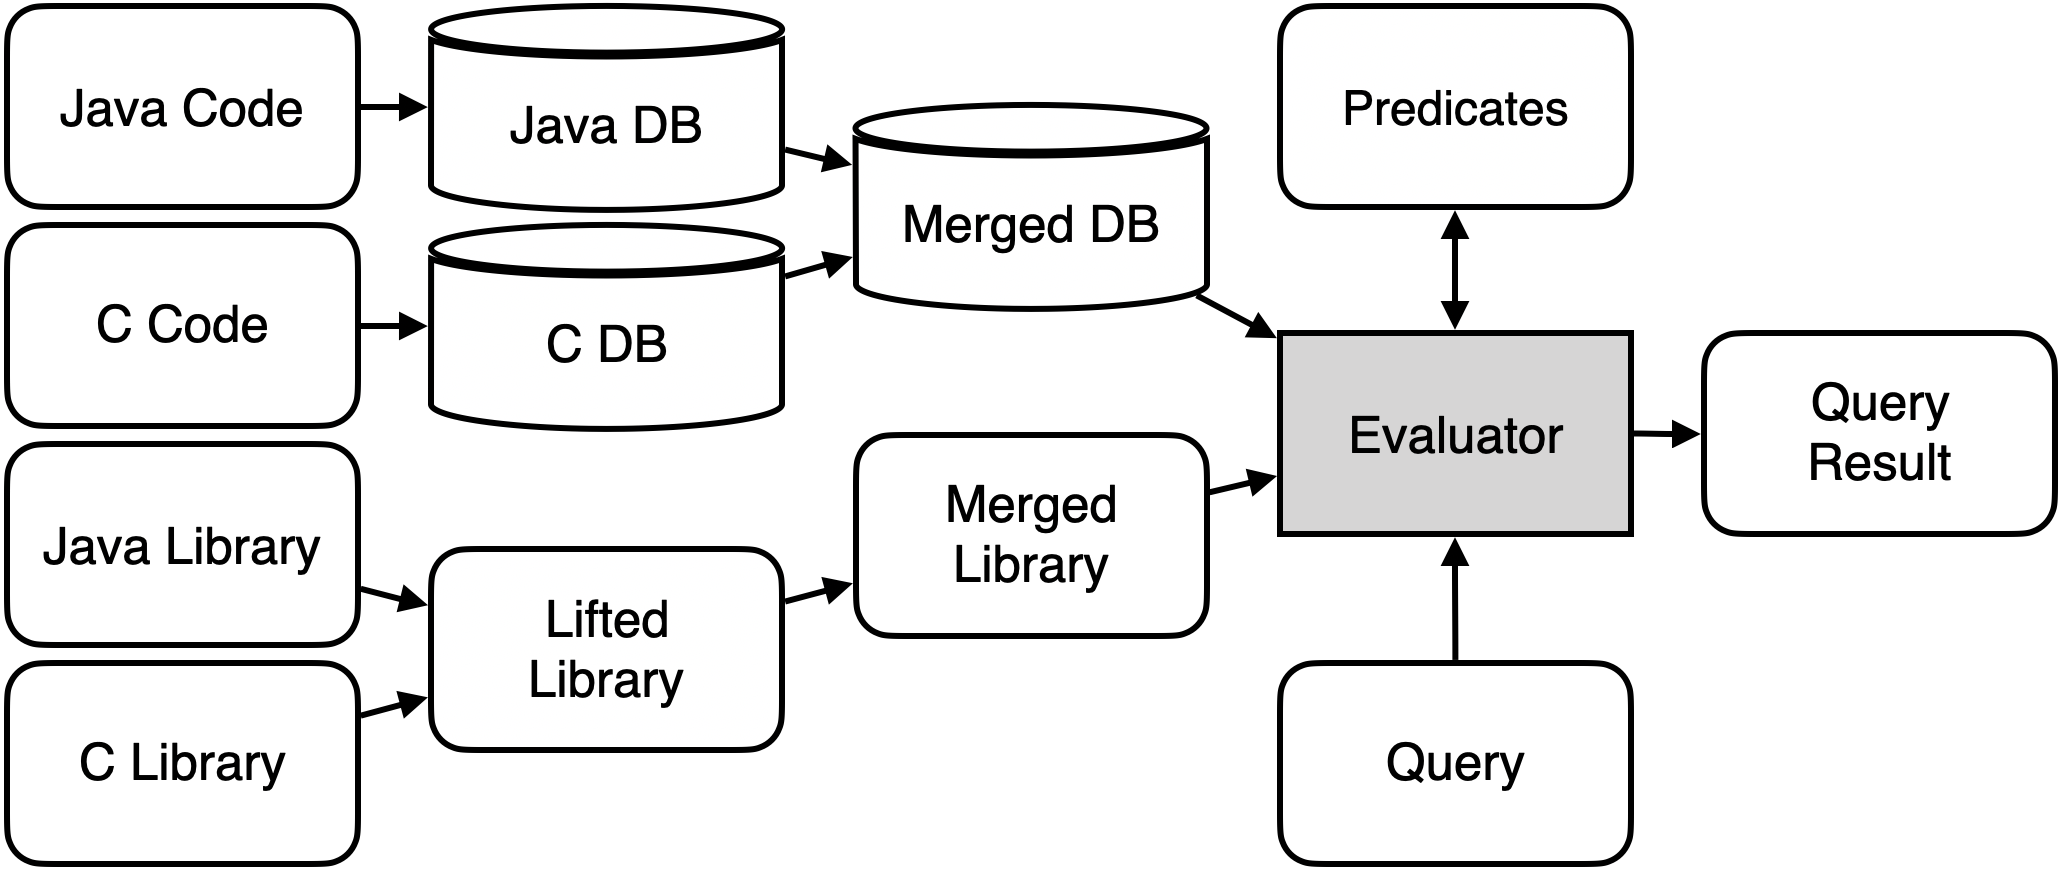
\includegraphics[width=0.47\textwidth]{img/codeql}
  \caption{Overall structure of JN-QL}
  \label{fig:codeql}
\end{figure}

\section{Implementation}\label{sec:impl}
In this section, we present JN-QL, a prototype implementation of our
approach to a declarative static analysis for multilingual programs,
in the case of dataflow analysis for JNI programs using CodeQL~\cite{codeql}.

\subsection{CodeQL}
CodeQL is a static analysis engine that transforms source code
programs into databases, and performs analysis by evaluating queries
written in the declarative language called QL (Query Language).
In QL, one can define rules by defining ``predicates'' or ``classes.''
For example, the following QL code defines the predicate \codeql{isOneTwoThree}:
\begin{lstlisting}[style=codeql,xleftmargin=2.5em]
predicate isOneTwoThree(int n) {
  n = 1
  or
  n = 2
  or
  n = 3
}
\end{lstlisting}
and the following definition defines the class \codeql{OneTwoThree}:
\begin{lstlisting}[style=codeql,xleftmargin=2.5em]
class OneTwoThree extends int {
  OneTwoThree() { // characteristic predicate
    this = 1
    or
    this = 2
    or
    this = 3
  }
}
\end{lstlisting}
A class defines a set of elements that satisfy the predicate called
``\codeql{characteristic predicate}.''
For more information about QL, one can refer to \citet{ql2016}'s paper
or the official document~\cite{codeql}.

Figure~\ref{fig:codeql} presents the overall structure of JN-QL.
First, it generates databases for both languages, C\footnote{
Even though JN-QL analyzes JNI programs written in Java and both C and
C++, this paper refers to C only fore presentation brevity.} and
Java, and merges them to one database.  This corresponds
to the step of extracting syntactic datafacts from source code programs.
Then, we merge the common datafacts and rules in both languages,
which are parts of their libraries that CodeQL provides, into one merged library.
Finally, using the merged database and merged library, a user can write a query to
perform a client-analysis, and evaluate it to produce its analysis result.

\subsection{Creating Databases}
For compiled languages such as C and Java, CodeQL generates their database
by compiling source programs.  When a compiler compiles a program,
CodeQL monitors the compiler to extract necessary information and
creates a database with the extracted information.
CodeQL creates a database for a single language in two steps:
1) it stores the extracted information from a compiler in a trap
file, a human readable file format, and 2) it fianlizes trap files
into databases in the binary format. For example, the
following shows a sample trap file:

\begin{lstlisting}[style=java,numbers=none]
#10017=@"class;hello.HelloJNI"  ...
#10044=@"type;int"
primitives(#10044,"int")  ...
#10061=@"callable;{#10017}.java_callback({#10044}){#10044}"  ...
#10067=@"params;{#10061};0"
params(#10067,#10044,0,#10061,#10067)
paramName(#10067,"java_callback_param")
\end{lstlisting}
which describes the parameter information about \javacode{java\_callback}.

\begin{figure}[t]
  \centering
  \vspace{2mm}
  \begin{subfigure}[t]{0.5\textwidth}
\begin{lstlisting}[style=codeql,xleftmargin=2.5em]
class Node extends TNode { ... }
predicate simpleLocalFlowStep(Node from, Node to) {
  exprToExprStep_nocfg( // Expr -> Expr
    from.asExpr(),
    to.asExpr()
  )
  or ...  // Assignment -> LValue post-update node
}
\end{lstlisting}
    \vspace*{-.5em}
    \caption{c/dataflow/internal/DataFlowUtil.qll}
  \end{subfigure}
  \begin{subfigure}[t]{0.5\textwidth}
\begin{lstlisting}[style=codeql,xleftmargin=2.5em]
class Node extends TNode { ... }
predicate simpleLocalFlowStep(Node node1, Node node2) {
  // Variable flow steps through
  // adjacent def-use and use-use pairs.
  exists(SsaExplicitUpdate upd |
    upd.getDefiningExpr().(VariableAssign).getSource()
      = node1.asExpr() or
    upd.getDefiningExpr().(AssignOp) = node1.asExpr()
  |
    node2.asExpr() = upd.getAFirstUse()
  )
  or ...  // Flow through this
}
\end{lstlisting}
    \vspace*{-.5em}
    \caption{java/dataflow/internal/DataFlowUtil.qll}
  \end{subfigure}
  \vspace*{-.5em}
  \caption{QL libraries for C and Java}
  \label{fig:qll}
\end{figure}

To create a single database for both C and Java, JN-QL maintains
a separate trap file for each language and then merges them.
Note that both trap files may have tables with the same name.
To avoid name conflicts in a merged database, we add a
language-specific prefix to each table.
For example, if both trap files have tables named \codeql{@expr},
we rename the table from C as \codeql{@c\_expr},
and the table from Java as \codeql{@java\_expr"}.
After renaming such tables, we can safely finalize the trap files into
databases on which queries can be evaluated.

\subsection{Lifting Libraries}

CodeQL provides various libraries for C and Java, including
pre-defined predicates and classes for users to implement their own analyses.
A dataflow analysis library is such a library, which supports both C and Java.
For example, Figure~\ref{fig:qll} shows sample QL libraries for C and Java,
which uses the same class name \ccode{Node} and the same predicate
name \ccode{simpleLocalFlowStep}.
However, even with the same name, the class \ccode{Node} in C and the
class \javacode{Node} in Java are different classes, which are incompatible.
The same applies to the predicate \ccode{simpleLocalFlowStep}.
In other words, we can not use the class \ccode{Node} in C as an
argument of the predicate \javacode{simpleLocalFlowStep} in Java or vice versa.

To make classes and predicates in C and Java become compatible,
we lift each library to the common level.
First, we encapsulate each of the original dataflows in a CodeQL
module named C and JAVA so that we can distinguish the original
classes and predicates by lifted ones.
We can lift a class by first defining a sum type, denoting that
the lifted class comes either from C or Java, and then making the
lifted class be of that type.  We also implement two member predicates
that can cast the lifted class into the C or Java class:
\begin{lstlisting}[style=codeql,xleftmargin=2.5em]
private newtype TNode =
  TJavaNode(JAVA::Node n)
  or
  TCNode(C::Node n)
class Node extends TNode {
  JAVA::Node asJava() {
    this = TJavaNode(result)
  }
  C::Node asC() {
    this = TCNode(result)
  }
  ...
}
\end{lstlisting}
Similarly, we can lift a predicate by combining two original predicates with
the \codeql{or} connective. For each original predicate, we cast down
each of the arguments and return values to the class of its corresponding language:
\begin{lstlisting}[style=codeql,xleftmargin=2.5em]
predicate simpleLocalFlowStep(Node node1, Node node2) {
  JAVA::simpleLocalFlowStep(
    node1.asJava(), node2.asJava()
  )
  or
  C::simpleLocalFlowStep(
    node1.asC(), node2.asC()
  )
}
\end{lstlisting}
After lifting, lifted predicates show the equivalent behaviors as the
original ones if all the arguments are from the same language.


\subsection{Merging Libraries}
After the library is lifted, the last step is to extend some predicates to
reflect the semantics of interoperation between languages. The interaction from
Java to C, or C to Java are identified, and some predicates are extended to
model their behaviors. As an concrete example, Let's take a look how the predicate
named viableCallable can be extended.

\begin{figure}[t]
\begin{lstlisting}[style=codeql,xleftmargin=2.5em]
DataFlowCallable viableCallable(DataFlowCall c) {
  result.asJava() = JAVA::viableCallable(c.asJava())
  or
  result.asC() = C::viableCallable(c.asC())
  or
  result.asC() = viableCallableJ2C(c.asJava())
  or
  result.asJava() = viableCallableC2J(c.asC())
}
\end{lstlisting}
\caption{libray merge}
\end{figure}

The first two lines are result of lifting, and they take advantage of the
original predicates from dataflow library.  They handle the call edges from
Java to Java, and from C to C.

Next two lines are the result of merging library, and they are responsible for
inter-language call edges.  The predicate "viableCallableJ2C" finds call edges
from Java to C, and the predicate "viableCallableC2J" finds call edges from
C to Java. These two call edges have different characteristic, and they
are implemented in different way.

\textbf{Java to C} The interaction from Java to C is done by Java code
calling native function in C, possibly with some arguments. The function
call target is determined in static manner. The target function should
follow the JNI naming convention, which is adding "Java\_" as prefix, 
followed by fully qualified name of class and additional "\_", to the
method name. For example, the target function name for the method call
cfunction would be Java\_fully\_\_qualified\_\_class\_\_name\_cfunction.
Based on this convention, we can define the predicate viableCallableJ2C
so that f = viablaCallableJ2C(m) holds when f.toString() = "Java\_" + 
m.className() + "\_" + "m.toString() holds.

\textbf{C to Java} The interaction from C to Java is more complex, and
requires more detailed implementation. The biggest difference is that
the method call from C to Java requires the run-time value of variables.
First, C calls the interface function "GetMethodID(name, sig)" to get "method
ID" of the method whose name matches the first argument, and the type signature
matches the second argument passed to this function. This method id is stored
at a variable, say "mid", and actual method call is done by calling another
interface function, "Call<type>Method(obj, mid, args...)". Calling this interface
function corresponds to call the method that mid indicates, with the "this object" as
obj, and the arguments as args.

In order to correctly handle this method call, we have to answer these
questions: "what string values does 'name' or 'sig' have when GetMethodID is
called", and "what method ID value does 'mid' have when Call<type>Method is
called". Note that what we need to answer to this question is the dataflow
analysis. Although inter-language dataflow is needed to soundly answer to the
questions, in practice intra-language dataflow analysis is enough in most
situations. Therefore, we implemented two "inner-flow" analysis module for C,
which find all the dataflow from string literal to the argument of interface
function, and the dataflow from interface function call result to the argument
of interface function. Based on these two modules, we can implement the
predicate viableCallableC2J by connecting the call edge from "Call<type>Method"
call to the method m, if there is a flow to mid from call to "GetMethodID", and
string values that flow into name argument and sig argument of the "GetMethodID"
corresponds with that of method m.

Other than the predicate viableCallable, there are also other predicates that
are extended. Most of them are specialized "step" predicates, where the purpose
of extension is to consider other JNI interface functions, such as
findClass or GetFieldID. The extensions are done in similar as handling
call from C to Java mentioned above.
